\chapter{Réalisation logicielle}

    % =============== API de commande de l'ARDrone ===================
    \section{API de commande de l'ARDrone}
        Étant un objet grand public, l'ARDrone bénéfice d'une communauté active. Cette communauté est à l'origine d'un certain nombre d'API de commande que ce soit en Javascript, C\#, Java ou C. Le SDK OptiTrack étant en C, nous avons recherché des API étant également codée en C afin de pouvoir fusionner facilement les deux outils.\\

        Nos recherches nous ont menées au SDK de Parrot (la marque du drone), intégralement écrit en C et embarquant toutes les fonctionnalités nécessaires. Cependant, la phase de compilation de cette librairie s'est trouvée être très fastidieuse que ce soit sur Linux ou sur Windows. La raison est le nombre important de librairies tierces utilisé par le SDK du drone pour gérer les flux vidéo, les threads, ou encore les contrôleurs. Après avoir passé du temps a travaillé dessus et à tenter d'en extraire les fonctionnalités de pilotage du drone, il s'est avéré plus simple d'en écrire une nouvelle en C++, exclusivement dédiée au contrôle de l'appareil. De ce fait, nous perdons les informations fournies par le drone (télémétrie, flux vidéo), mais gagnons en simplicité et comprenons mieux ce que nous faisons.

        % ------------- API réalisée -----------------
        \subsection{API réalisée}
            Le drone se contrôle assez simplement, mais selon un formalisme strict. Pour interagir avec, il faut se connecter en UDP sur le port 5556 de l'appareil (192.168.1.1). Une fois connecté, il faut envoyer des commandes \textbf{AT} au minimum toute les 50 ms pour maintenir la connexion active. Les commandes diffèrent selon la nature de l'instruction:
            \begin{itemize}
                \item \textit{AT*FTRIM=seq} pour calibrer le drone, avec \textit{seq} le numéro du message;
                \item \textit{AT*COMWDG=seq} pour maintenir la connexion sans donner d'instruction;
                \item \textit{AT*REF=seq,value} pour faire décoller/atterrir ou stopper le drone en urgence…
            \end{itemize}
            L'API réalisé propose donc un objet ARDrone contrôlant un thread de communication avec le drone et plusieurs méthode simple comme \textit{takeOff()}, \textit{move()} ou \textit{land()}.


    % =============== Récupération des données 3D ===================
    \section{Récupération des données 3D}

        % ----------- Client-serveur ----------------
        \subsection{Client-serveur}
            Le système mis en place n'est pas simple à appréhender puisqu'il nécessite l'utilisation d'un client-serveur au sein du même PC\@. Le diagramme~\ref{fig_organisation_systeme} permet de mieux comprendre.

            \begin{figure}[h]
                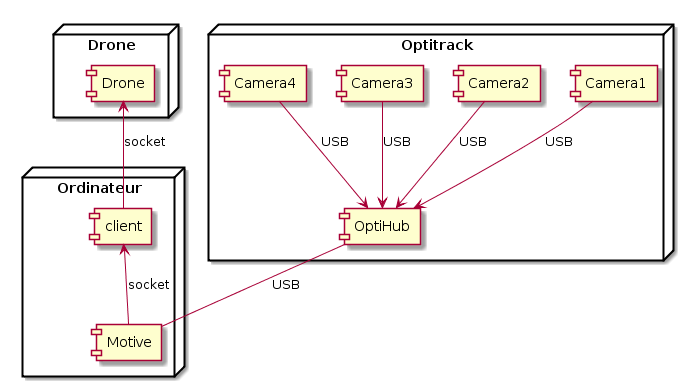
\includegraphics[width=13cm]{images/diagramme_Composant.png}
                \caption{Organisation du système}
                \label{fig_organisation_systeme}
            \end{figure}

            La communication entre Optitrack et notre programme est assurée par la librairie NatNet disponible dans le SDK Optitrack. Les informations envoyées par Motive sont par exemple le nombre de RigidBody ainsi que leur position/orientation dans l'espace.


    % =============== Gestion des déplacements du drone ===================
    \section{Gestion des déplacements du drone}

        % ----------- Pilotage à l'aide de la coque ----------------
        \subsection{Pilotage à l'aide de la coque}
           La première fonction mise en œuvre durant ce PAO a été le pilotage du drone à l'aide d'une seconde coque de drone. Aucun asservissement nécessaire, nous demandions simplement au drone de se pencher dans le même sens que la coque de commande. Nous n'avions donc pas de contrôle sur l'altitude à ce moment. \\

           Une fois la commande du drone finalisée, nous avons pu implémenter un correcteur P (proportionnel) sur les deux axes horizontaux, sur le lacet, et sur l'axe vertical. Ainsi lorsque nous placions la coque de commande à un endroit dans la pièce, le drone s'y rendait. Le correcteur P seul étant peu performant, le drone avait des difficultés à stabiliser sa position.

        % ----------- Trajectoire par points de passage ----------------
        \subsection{Trajectoire par points de passage}
            Une fois l'asservissement en position implémenté grâce à la coque de contrôle, nous avons été en mesure d'enregistrer plusieurs positions successives dans l'espace. Ainsi, le drone a pu effectuer des trajectoires passant par ces positions pré-enregistrées. Pour que le drone ne tente pas indéfiniment d'atteindre une position précise, nous avons intégré une zone d'erreur de quelques cm afin de considérer la position comme atteinte.

        % ----------- Amélioration de l'asservissement ----------------
        \subsection{Amélioration de l'asservissement}
            Le correcteur P seul entraînant beaucoup d'instabilités, nous avons décidé d'implémenter un correcteur PID (Proportionnel, Intégrateur, Dérivé) complet sur chaque axe. Nous nous sommes tout d'abord heurtés à l'implémentation de ces derniers dans un contexte discret, puis au choix des constantes. Finalement, nous avons décidé de n'utiliser que les corrections P et D car notre drone ne possédait pas d'erreur statique. Les valeurs des constantes P et D on été déterminées expérimentalement.
